\chapter{Выбор метода решения}
\label{chap:methods}
    \section{Подходы к решению задачи}
    \par
        Для решения данной задачи предлагается действовать по данному алгоритму:
        \noindent
        \begin{enumerate}
            \item Предобработка данных
            \item Отбор признаков
            \item Решение задачи классификации
            \item Адаптация классификатора
        \end{enumerate}
        
        \begin{figure}[h!]
                \centering
                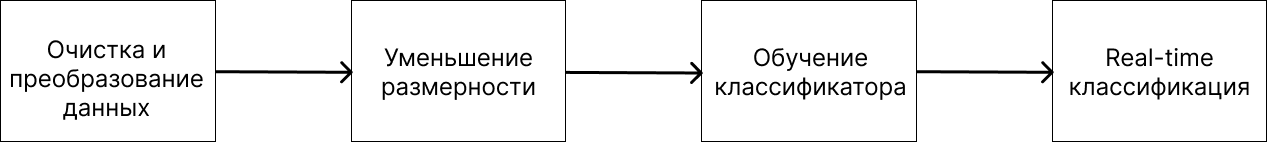
\includegraphics[scale=0.7]{pictures/logic.png}
                \caption{Алгоритм решения}
                \label{fig:my_label}
            \end{figure} 
    \newpage
    \section{Формулировка требований к решению} \\
        \paragraph{Необходимые свойства решения:}
         \\
        \begin{itemize}
            \item Оптимальность по времени выполнения
            \item Реальные требования к вычислительной мощности обрабатывающего устройства
            \item Масштабируемость композиции алгоритмов
            \item Отсутствие вычислений для нового образца по всем данным
            \item Возможность объединения алгоритмов для потоковой обработки сигналов
            \item Возможность дообучения на неразмеченных данных
            \item Сохранение модели для дальнейшего использования
            \item Возможность классификации без хранения обработанных ранее данных \\ \\
        \end{itemize}
        
    \newpage    
    \section{Методы решения}
    
        \paragraph{Выбор алгоритма для преобразования RAW сигнала} 
            \noindent \\
            
            \noindent
            Есть несколько вариантов преобразований RAW сигнала, а также множество их комбинаций. \\ \\
            В данной работе рассмотрены:
            \begin{itemize}
                \item FFT -- Fast Fourier transform -- алгоритм ускоренного вычисления дискретного преобразования Фурье.\\
                Данный алгоритм, в отличие от прямого дискретного преобразования Фурье, выполняющегося за $O(N^2)$, имеет асимптотику $O(N log(N))$.
                \item Разложение сигнала на модуль и аргумент.
                \item Разложение на действительную и мнимую части. \\
            \end{itemize} \\
        \paragraph{Выбор алгоритма для уменьшения размерности}
        \noindent \\
    
            \noindent 
            Для данной задачи необходимо значительно уменьшить размерность признакового пространства, по минимуму потеряв важную информацию об RF-Fingerprint устройства.\\ \\ 
            Может понадобиться не просто убрать менее значимые признаки, а создавать композиции из имеющихся признаков для минимальных потерь. Этой способностью обладают автоэнкодеры на основе нейронных сетей. \\ \\
            В данной работе рассмотрены:
            \begin{itemize}
                \item Алгоритм проекции на 2-мерное признаковое пространство -- TSNE
                \item Отбор признаков с помощью алгоритма Random Forest
                \item Встроенный автоэнкодер MATLAB
                \item Автоэнкодер, построенный с помощью библиотеки tensorflow.keras
                \item Permutation importance из библиотеки sklearn.inspection \\
            \end{itemize}
            
    
        \paragraph{Выбор алгоритма для классификации}
        \noindent\\
        
            \noindent
            Для данной задачи необходимо достаточно точно классифицировать зашумленные данные, обладающие признаками со сложной внутренней зависимостью. \\ \\
            Алгоритмы классификации, которые подходят для решения данной задачи должны быть быстродействующими, нетривиальными и помехоустойчивыми. \\ \\
            В данной работе рассмотрены: 
            \begin{itemize}
                \item Decision Tree -- Решающее дерево -- алгоритм, основанный на разделении по значению признаков для построения дерева
                \item Random Forest -- Случайный лес -- композиция решающих деревьев, более устойчивая к переобучению
                \item Multilayer Perceptron -- полносвязная нейронная сеть построенная с помощью библиотеки sklearn.sknn
                \item CatBoostClassifier -- open source классификатор от компании Yandex
            \end{itemize}   
            
            %про всякие алгоритмы